\section{Results}
    Will contain a presentation of the various spectral fitting results in figures and tables.

    To perform fitting of NICER data \cite{orio2022nicer}

    \subsection{Observed count rates}
    In figure \ref{fig:all-counts}, we present a comparison of count rates derived from the multiple observations listed in table ***. Figure \ref{fig:all-counts:unnorm} serves to illustrate the variability of flux across different observation epochs, with count rates plotted on a logarithmic scale. This visualization provides insights into the temporal evolution of X-ray emission from MR Vel.

    \begin{figure*}[!htb]
        \centering
        \begin{subfigure}[b]{0.45\textwidth}
            \centering
            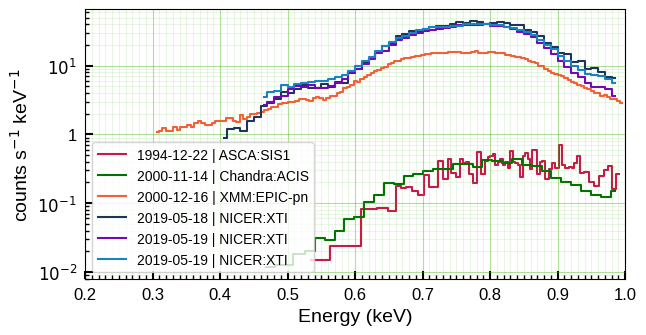
\includegraphics[width=\textwidth]{figures/ldata/mr-vel-counts_all-obs.png}
            \caption{Comparison of flux from all observations from their count rates plotted to scale}
            \label{fig:all-counts:unnorm}
        \end{subfigure}
        \hfill
        \begin{subfigure}[b]{0.45\textwidth}
            \centering
            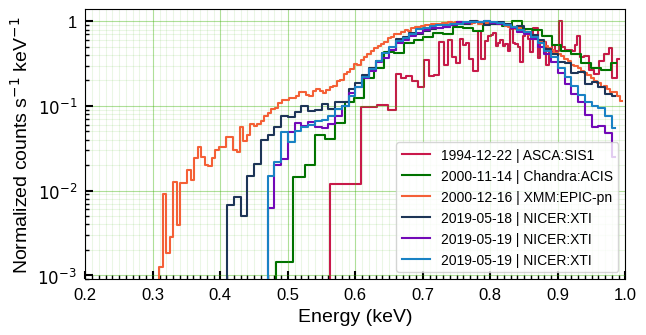
\includegraphics[width=\textwidth]{figures/ldata/mr-vel-normcounts_all-obs.png}
            \caption{Normalized count rates from all observations show varying responses to supersoft X-rays}
            \label{fig:all-counts:norm}
        \end{subfigure}
        \caption{Count rates from observational dataset}
        \label{fig:all-counts}
    \end{figure*}
    
    Concurrently, in figure \ref{fig:all-counts:norm}, the count rates are normalized to the range of 0 to 1 using \textit{min-max normalization}. This visualization accentuates the relative sensitivity of more recent observations to supersoft X-ray photons emitted by MR Vel. The sub-plot shows that in recent observations the supersoft X-ray features are discernibly enhanced. This might be suggestive of improved observational capabilities or heightened sensitivity to the emitted X-ray flux.
    
    Together, these visualizations offer a nuanced understanding of the flux variability and observational sensitivity trends exhibited by MR Vel across different observation epochs, contributing to the broader understanding of its X-ray emission characteristics.

    \subsection{Unfolded spectra}
    In figure \ref{fig:all-uf}, the unfolded spectrum, which is obtained after fitting the data to the best-fit model, is displayed. Observations in panels \ref{fig:all-uf:12-24} and \ref{fig:all-uf:24-36} reveal features which are indicative of the presence of elemental absorption edges.
    
    \begin{figure*}[!bht]
        \centering
        \begin{subfigure}[b]{0.45\textwidth}
            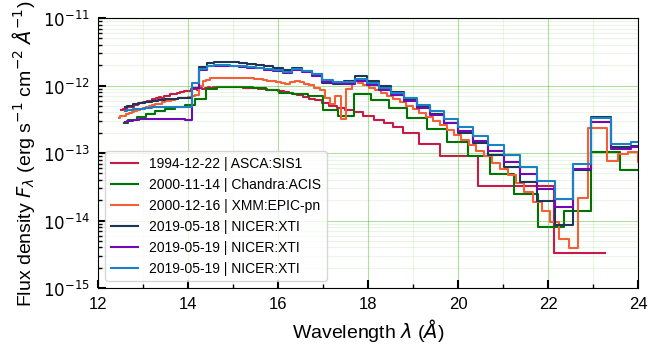
\includegraphics[width=\textwidth]{figures/eufspec/mr-vel-uf_all-obs_12-24.png}
            \caption{Unfolded spectra after model fitting in the range 12 \AA - 24 \AA}
            \label{fig:all-uf:12-24}
        \end{subfigure}
        \hfill
        \begin{subfigure}[b]{0.45\textwidth}
            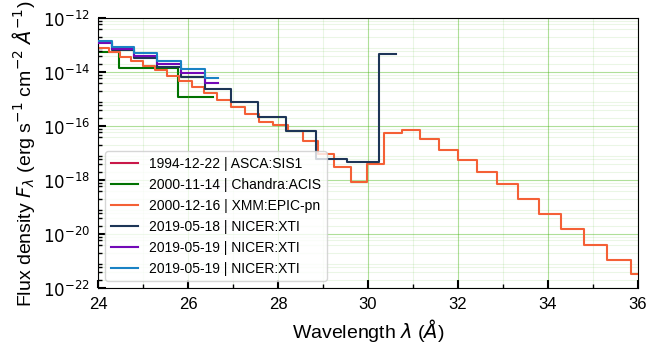
\includegraphics[width=\textwidth]{figures/eufspec/mr-vel-uf_all-obs_24-36.png}
            \caption{Unfolded spectra after model fitting in the range 24 \AA - 36 \AA}
            \label{fig:all-uf:24-36}
        \end{subfigure}
        \caption{Unfolded spectra after model fitting}
        \label{fig:all-uf}
    \end{figure*}

    \subsection{Presence of elemental absorption edges}
    Four elemental absorption edges were detected upon the inspection of the unfolded spectra obtained from the best fitting model on all the observations. These absorption edges, belonging to N, O, Ne and Fe, are overlaid on the unfolded spectra and displayed in figure \ref{fig:all-uf:abs-edges}.
    \begin{figure*}[!htb]
        \centering
        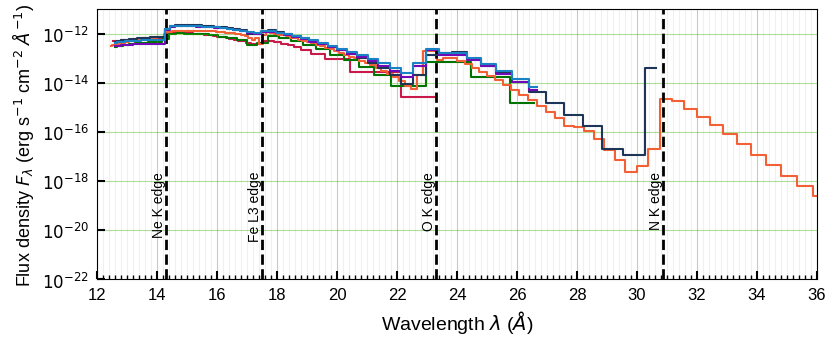
\includegraphics[width=0.8\textwidth]{figures/eufspec/mr-vel-uf-ang_abs-edge.png}
        \caption{Unfolded spectra with overlaid elemental absorption edges}
        \label{fig:pn-uf:abs-edges}
    \end{figure*}

    Because the best-fitted spectrum obtained from the EPIC-pn instrument of XMM-Newton spans the widest range of wavelengths, known absorption edges \cite{bearden1967reevaluation,juett2006high} were identified in the vicinity of the absorption edges in figure \ref{fig:all-uf:abs-edges}. Then they were overlaid on the unfolded spectrum obtained from the EPIC-pn observation.

    \begin{figure*}[!bht]
        \centering
        \begin{subfigure}[b]{0.45\textwidth}
            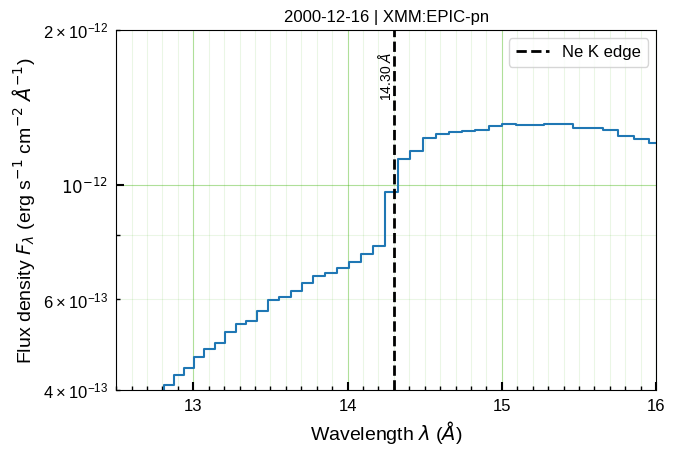
\includegraphics[width=\textwidth]{figures/eufspec/mr-vel-XMM-EPIC-pn-uf-Ne-edges.png}
            \caption{Ne K absorption edge at 14.302 \AA}
            \label{fig:pn-uf:Ne-edges}
        \end{subfigure}
        \hfill
        \begin{subfigure}[b]{0.45\textwidth}
            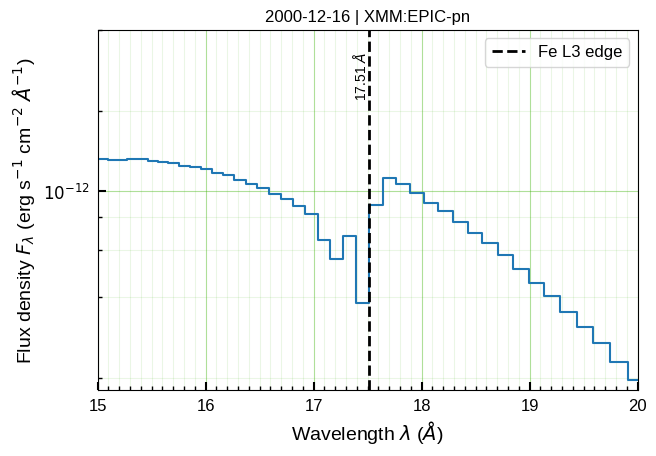
\includegraphics[width=\textwidth]{figures/eufspec/mr-vel-XMM-EPIC-pn-uf-Fe-edges.png}
            \caption{Fe L$_3$ absorption edge at 17.509 \AA}
            \label{fig:pn-uf:Fe-edges}
        \end{subfigure}
        \begin{subfigure}[b]{0.45\textwidth}
            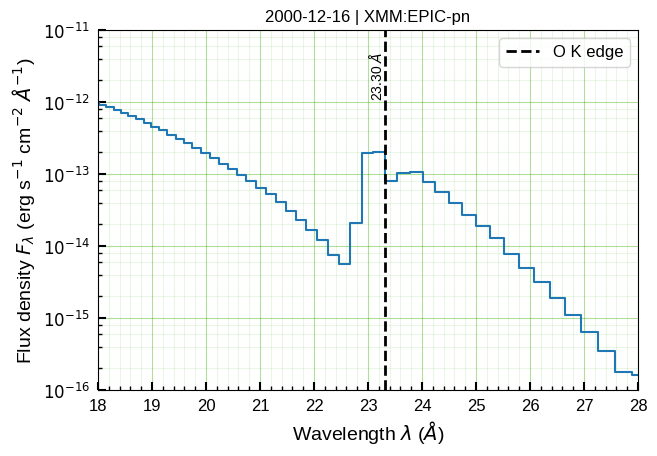
\includegraphics[width=\textwidth]{figures/eufspec/mr-vel-XMM-EPIC-pn-uf-O-edges.png}
            \caption{O K absorption edge at 23.305 \AA}
            \label{fig:pn-uf:O-edges}
        \end{subfigure}
        \hfill
        \begin{subfigure}[b]{0.45\textwidth}
            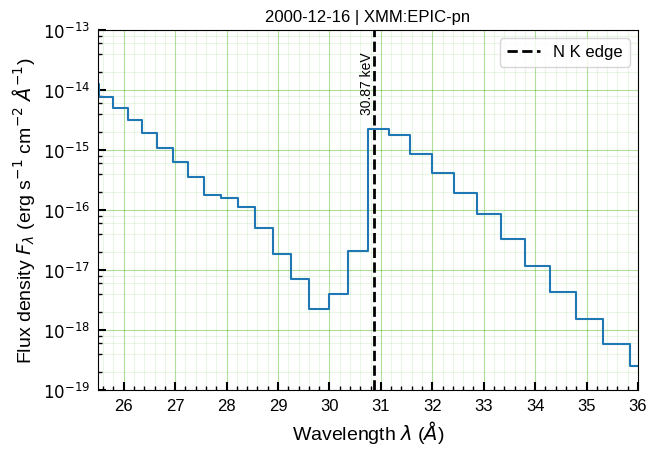
\includegraphics[width=\textwidth]{figures/eufspec/mr-vel-XMM-EPIC-pn-uf-N-edges.png}
            \caption{N K absorption edge at 30.873 \AA}
            \label{fig:pn-uf:N-edges}
        \end{subfigure}
        \caption{Absorption edges for N, O, Ne and Fe overlaid on the unfolded spectrum for EPIC-pn observation}
        \label{fig:pn-uf:abs-edges}
    \end{figure*}
